\IEEEPARstart{A}{} continuaci\'on se detallan todos los experimentos realizados
en este trabajo y sus resultados.

\par A diferencia de trabajos previos, la experimentaci\'on de este trabajo es
mucho m\'as explorativa que basada en hip\'otesis a confirmar. Claramente, al
comenzar la experimentaci\'on se tuvieron algunas hip\'otesis (detalladas a
continuaci\'on), pero se comenz\'o esta tarea m\'as con un objetivo de observar
que ocurre con los m\'etodos propuestos seg\'un algunas variables que fueron
identificadas.

\par A su vez, el dominio de este trabajo es m\'as subjetivo, si se quiere, que
los trabajos previos. Es decir, al interpolar cuadros (o \emph{frames}) de un
video, nos interesa como es la percepci\'on de la audiencia del mismo. ¿Se nota
la interpolaci\'on?¿Da una sensaci\'on anormal?¿No se nota, quiz\'as?.
B\'asicamente: el resultado obtenido, ¿es bueno?. Claramente esto es muy
subjetivo y dependiente, entre otras cosas, de la persona que emite el juicio.
As\'i pues, se tuvo que buscar alguna forma de comparar los distintos m\'etodos
de la forma m\'as objetiva posible. Pero tampoco se quizo dejar de lado este
an\'alisis ''subjetivo'', que al fin y al cabo, es el m\'as importante.

\par A lo largo de esta secci\'on comenzaremos primero enunciando las
hip\'otesis que se pudieron enunciar antes de comenzar, la explicaci\'on de las
variables con las que se experiment\'o (derivadas a partir de las hip\'otesis),
para luego pasar a la experimentaci\'on misma (con un m\'inimo an\'alisis de
correctitud), d\'onde se analizan los aspectos cu\'antitativos y cualitativos
(y como se a explicado, algunos de estos \'ultimos de manera subjetiva).
Finalmente, realizamos una an\'alisis breve de los \emph{artifacts} frutos de
los videos interpolados y terminamos esta secci\'on indicando ciertos trabajos
a futuros que podr\'ian ser de inter\'es.

%---------------------------------------------------------------
\subsection{Hip\'otesis}
En esta parte del trabajo se explican algunas de las hip\'otesis
que pudieron ser formuladas al pensar en el problema. Como ya se ha dicho, la
naturaleza de este trabajo ha sido m\'as exploratoria, pero a\'un as\'i se
comenz\'o el mismo con algunas conjeturas y nociones de lo que deb\'ia ocurrir.

\begin{enumerate}
    \item\begin{LaTeXdescription}
        \item[Hip\'otesis] saraza

        \item[Motivaci\'on] saraza
    \end{LaTeXdescription}
\end{enumerate}


%---------------------------------------------------------------
\subsection{Variables Identificadas para la Experimentaci\'on}
\IEEEPARstart{A}{} partir de las hip\'otesis enunciadas, se determinaron
ciertas caracter\'isticas y par\'ametros que posiblemente afecten a la calidad
de las interpolaciones aplicadas a los videos. Estas son:

\begin{LaTeXdescription}
    \item[Frames Interpolados]

    \item[M\'etodo de Interpolaci\'on]

    \item[Tama\~no de Bloque (splines)]

    \item[Resoluci\'on del Video]

    \item[Duraci\'on del Video]

    \item[Tipo Movimiento grabado por la C\'amara]

    \item[Tipo de Movimiento de la C\'amara]
\end{LaTeXdescription}

\par Estas son algunas de las variables que se podr\'ian en tener en cuenta (en
particular las que se tuvieron en cuenta en este trabajo), pero no son las
\'unicas. Por dar un ejemplo, una variable con la que no se trabaj\'o fue con
los videos que cambi\'an de c\'amara, donde se pas\'a de un tipo de im\'agen a
otra de form\'a rotunda en frames contiguos (podr\'ia haber alg\'un tipo de
transici\'on tambi\'en, que ser\'ia otro caso a estudiar). Fue meramente por
cuestiones de tiempo que se decidi\'o limitar el enfoque de este trabajo a las
variables/par\'ametros enunciados.


%---------------------------------------------------------------
\subsection{Metodolog\'ia de Experimentaci\'on}
Durante la experimentaci\'on, y dada la naturaleza de la misma,
se sigui\'o una misma metodolog\'ia para recabar la informaci\'on necesaria para
ser luego analizada.

\par En primer lugar se decidi\'o trabajar con im\'agenes en escala de grises o,
coloquialmente llamado \emph{blanco y negro}. Esto es as\'i ya que dentro del
alcance de nuestro trabajo, estamos estudiando (principalmente) la correctitud
de los frames interpolados. Si se tuvieran en cuenta los colores, se tendr\'ia
la complicaci\'on del error agregado de interpolar los canales de colores por
separado, lo cual escapa a los objetivos del trabajo (adem\'as de tener la
limitante del tiempo para realizar este trabajo.). Resumiendo, se tom\'o esta
decisi\'on para simplificar y enfocar m\'as el an\'alisis a realizar.

\par La forma en la que se presentar\'an los resultados m\'as adelante nada
tiene que ver con el orden en el que se realiz\'o la experimentaci\'on.

\par De la secci\'on anterior se puede observar que existen dos variables que
nos indican (o limitan) los tipos de videos con los que trabajaremos. Estas dos
variables no son otra que las diferentes combinaci\'on del tipo de movimiento
filmado y de la c\'amara que realiza la grabaci\'on. As\'i pues, se termin\'o
teniendo cuatro combinaci\'ones posibles: \emph{c\'amara fija-im\'agen fija},
\emph{c\'amara fija-im\'agen m\'ovil}, \emph{c\'amara m\'ovil-im\'agen fija} y
\emph{c\'amara m\'ovio-im\'agen m\'ovil}\footnote{Existen matices en estas
combinaciones. Por ejemplo, \emph{la suavidad} de los movimientos, que podr\'ian
variar en intensidad yendo de suaves a bruscos. Nuevamente, por cuestiones de
tiempo se decidi\'o no incursionar en estos aspectos.}.

\par Nos interesa comparar de manera imparcial los métodos utilizados,
utilizando alguna medida de cuánto se acercan a ``la realidad'': en nuestro
caso, a lo que habría captado una cámara de alta frecuencia. Pero para hacerlo
haría falta tener dos videos del mismo evento, filmados desde el mismo punto,
uno con una cámara de alta frecuencia y otro con una normal. Como las cámaras
ocupan un espacio, esto es físicamente imposible\cite{wiki_impenetrability}. Lo
que haremos, en su lugar, para comparar los métodos, será ``descartar'' frames
de un video (normal o no) y darle este nuevo video ``recortado'' como entrada a
nuestros métodos de interpolación. La comparación entre el resultado y el video
original nos dará una aproximación de cuán ``acertados'' son nuestros métodos
para siumlar lo que ocurre entre dos frames de un video cualquiera.

\par Entonces, para cada una de las categor\'ias de videos, se efectu\'o la
interpolaci\'on con los 3 m\'etodos expuestos y todas sus posibles
combinaciones de par\'ametros (cantidad de frames a interpolar entre frame y
frame, y en el caso de spline el tama\~no de bloque.), para luego poder hacer
un an\'alisis objetivo de la calidad de los frames interpolados resultantes.
Para realizar el descarte arriba mencionado, lo que se hizo fue remover de los
videos originales una cantidad calculada\footnote{En base a la cantidad de
frames a interpolar.} de frames antes de interpolar el mismo.

\par Luego se realizan los an\'alisis de los m\'etodos independientemente de los
dem\'as m\'etodos, es decir que analizamos los resultados obtenidos de cada
m\'etodo respecto de sus par\'ametros de entrada.

\par Continuamos realizando un an\'alisis de m\'etodo versus m\'etodo, para
los mismos par\'ametros (en el caso de splines, al tener 2 par\'ametros de
entrada\footnote{Cantidad de bloques a interpolar y tama\~no de bloque.} se
tuvieron que utilizar resultados obtenidos del an\'alisis del m\'etodo
realizado previamente).

\par Por \'ultimo, antes de terminar enunciando las conclusiones obtenidas para
el tipo de video estudiado, se generaron unos videos que realizan la
comparativa frame a frame de la diferencia entre el frame del video original y
su contraparte interpolada para luego ser estudiados (visualizado en forma de
\emph{heatmap}). La idea de esto es la de encontrar en que zonas de los frames,
respecto de lo que ocurre en el video, genera problemas para los m\'etodos
estudiados.

\par Para realizar la comparación, usaremos las definiciones de \texttt{ECM} y
\texttt{PSNR} ya dadas en la Introducción teórica, comparando frame a frame
entre los dos videos. Estas m\'etricas no son otras que las sugeridas por la
c\'atedra: el \emph{Error Cuadr\'atico Medio}\cite{mse} y el \emph{Peak Signal
to Noise Ratio}\cite{psnr}. El primero es una medida de error entre un valor
(en nuestro caso, un frame) estimado y lo que es estimado (el frame original).
Mientras que el \emph{PSNR} es un ratio que toma en cuenta el \emph{ECM} y el
valor m\'aximo siendo estimado\footnote{Oriundo del an\'alisis de se\~nales,
donde indica la relaci\'on entre la potencia m\'axima de una se\~nal y la
potencia del ruido que la afecta.}. Justamente el PSNR es utilizado para
cuantificar la calidad de la reconstrucci\'on de una se\~nal (o en nuestro
caso, de un frame), un alto valor del mismo del mismo indica mayor calidad de
la reconstrucci\'on (aunque se debe tener cierto cuidado en los casos donde
existe compresi\'on de datos involucrada, caso que no aplica a este trabajo).
Tambi\'en se usaron los valores medios, desv\'io est\'andard, m\'aximo y
m\'inimo del ECM para realizar comparaciones para el mismo m\'etodo y sus
diferentes par\'ametros, como as\'i tambi\'en entre los distintos m\'etodos.

\par Vale la pena aclarar que en las conclusiones generales es donde tambi\'en
se realiza un an\'alisis m\'as subjetivo, basado en la percepci\'on de los
autores de este trabajo. Claramente esta no es una muestra lo suficientemente
alta de las posibles audiencias de los videos, pero alcanza dado el objetivo
did\'actico del trabajo.

\par Para concluir con esta secci\'on, agregamos a su vez que se realizaron
otros experimentos m\'as puntuales para analizar los aspectos de correctitud de
los m\'etodos (m\'inimamente) y del tiempo de c\'omputo, como as\'i tambi\'en
una comparativa de como los m\'etodos se ven afectados seg\'un la variable
m\'as importante de todas: el video.

\par Los videos originales utilizados para la experimentaci\'on pueden
obtenerse en \url{https://drive.google.com/open?id=0B0RfkWV-4-XqMlhfa0Z2WUMtRTg}


%---------------------------------------------------------------
\subsection{Validaci\'on de la Implementaci\'on}
\IEEEPARstart{E}{n} este apartado, nos centramos a corroborar que los pasos de la implementaci\'on se dieron acorde a lo que cada m\'etodo visto propone. Para ello, creamos dos instancias en la cual se podr\'an visualizar con facilidad los cambios generados al aplicar el efecto de slowmotion. De hecho, uno de ellos se basar\'a de reproducir una sola im\'agen durante todo el video. El restante se basar\'a en observar el cambio entre los dos extremos que proporciona la escala de grises, es decir, de blanco a negro.
%---------------------------------------------------------------
\subsubsection{Blanco-Negro}

Nos situamos primero en el caso donde dicho video se comprende de dos tipos de frames, que es repetido una cierta cantidad de veces en un determinado tiempo. La particularidad de dichos frames, es que si se contempla \'estos como matriz, se confirma la igualdad en cada posici\'on del cuadro. Debido a que estamos trabajando sobre escala de grises, decidimos clasificar al tipo $A$ como un frame con todos sus p\'ixeles en negro (equivalente a $0$) y el tipo $B$ con p\'ixeles en blanco (equivalente a $255$).

En primer lugar, se seleccion\'o una im\'agen de esta caracter\'istica ya que nos podemos abstraer del procedimiento sobre el frame en conjunto. De esa manera, nos podemos enfocar en analizar cualquier posici\'on $(i,j)$. ¿Qu\'e utilidad nos brinda esto \'ultimo? El hecho de poder evaluar en detalle, el comportamiento del m\'etodo aferrado a nuestra implementaci\'on.

En segundo lugar, haber escogido dos valores que representan los extremos en la escala de representaci\'on, nos trae una mejor intuici\'on del resultado esperado. Con esto nos adelantamos a decir, que el video alentizado intentar\'a reflejar lo que sucede cuando se translada del tipo $A$ al $B$ mediante los frames interpolados.

Por \'ultimo, aclaramos que el video solo contendr\'a un cambio del frame de tipo $A$ al $B$, y ese mismo ser\'a definitorio.

\subsubsection*{Vecino m\'as cercano:}

Sabemos que su idea revoca en crear los cuadros intermedios copiando de un extremo u otro, tal como se explic\'o durante el desarrollo. Por ende, el resultado que \'este dar\'a al aplicarlo sobre el video, ser\'a bastante trivial. De hecho, lo \'unico que se podr\'a apreciar es la mayor duraci\'on del video resultante con respecto al original.

Pasamos a los resultados, que por la poca complejidad algor\'itmica que este m\'etodo implica, se validar\'a en brevedad a lo que se buscaba. 

\subsubsection*{\bf{Resultado:}}

Comprobamos que al decifrar los frames intermedios como matrices, \'estos se identificaron con su extremo m\'as cercano. Si al par\'ametro de cantidad de frames a adherir se le asignaba un n\'umero impar, luego en teor\'ia el valor del extremo derecho (en este caso, el blanco) tendr\'ia mayor presencia. Sin embargo, como la diferencia es de un solo frame adicional, no se not\'o nada en la pr\'actica debido a la cantidad de frames por segundo que corre el reproductor de video. 

En consecuencia, recolectamos la totalidad de frames del video en $slowmotion$ para comprobar si la implementaci\'on acert\'o con la distribuci\'on de cuadros intermedios.

\subsubsection*{Interpolaci\'on lineal:}

Nos inclinamos a una perspectiva que abarca mayor seriedad, ya que su comprobaci\'on se justificar\'a del lado matem\'atico. Si los u\'nicos dos puntos a trazar son el $(x0,y0) = (0,0)$ y $(x1,y1) = (1,255)$, luego la funci\'on a considerar tendr\'a la forma:

$f(x) = y0 + (y1-y0) * \frac{x - x0}{x1 - x0} = 255 * \frac{x}{255} = x$

Con esto \'ultimo, ya se puede considerar que tampoco traer\'a dificultad al momento de analizar correctitud.

\subsubsection*{\bf{Resultado:}}

Fuimos elevando el par\'ametro de entrada, agregando m\'as frames de por medio. De esta manera, el m\'etodo se encargaba de evaluar cada $f(x) = x$, con $x \in \{ \frac{1}{fr} ; \frac{2}{fr} \ldots ; \frac{fr}{fr} \}$. Como dicha funci\'on es creciente, notamos como efectivamente el avanze del video reflejaba el esclarecimiento del mismo, tomando valores de grises m\'as suaves hasta llegar al cero.

En este caso, mostramos un caso donde se le adicion\'o 10 frames, y luego comprobando al obtener la totalidad de im\'agenes, se verific\'o que los valores de los p\'ixeles intermedios, coincid\'ian con la funci\'on lineal en dicho punto. ( Ver figura \ref{fig:linealValidacion} ).


\begin{figure}[h!]
  \centering
    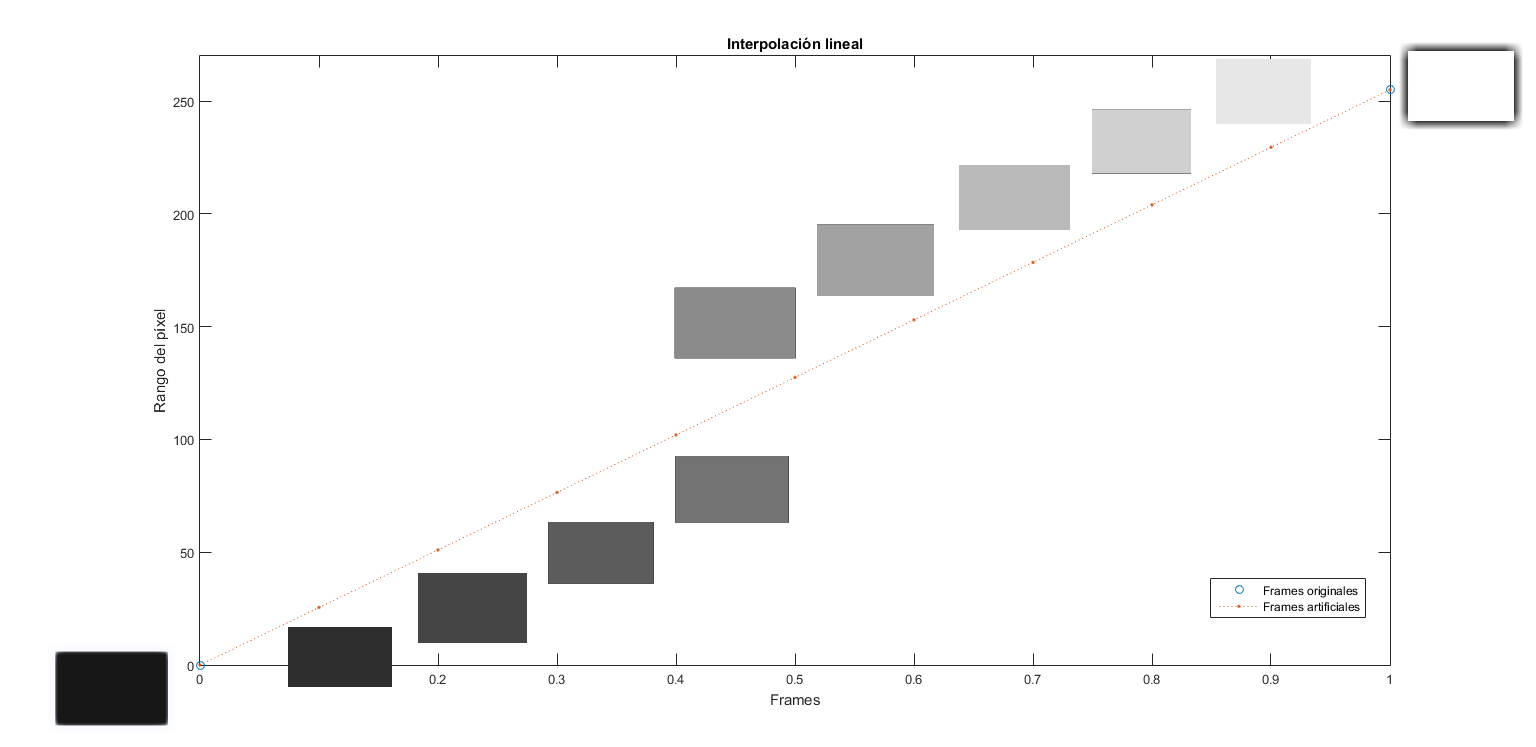
\includegraphics[width=0.75\textwidth]{GraficoLineal.png}
     \caption{Muestra del momento en que se realiza el cambio de blanco a negro, con sus respectivos frames intermedios}\label{fig:linealValidacion}
\end{figure}
\noindent

\subsubsection*{Splines}

Seguimos con la misma metodolog\'ia que con interpolaci\'on lineal, definiendo la funci\'on en cuesti\'on:

$f(x) = a (x - x0)^3 + b ( x - x0)^2 + c ( x - x0) + d$

Pero, ¿C\'omo hallamos los coeficientes del polinomio? Podr\'iamos por un lado, realizar las cuentas a papel y  de ah\'i seguir con el procedimiento de verificar con respecto a la implementaci\'on. Sin embargo, eso ser\'ia  bastante engorroso de realizar, por lo que optamos por usar un software inteligente cuyo nombre es $MatLab$. Usando la funci\'on $interpo1$ podemos obtener el valor de cualquier punto intermedio, en particular los que se evaluaron en nuestro programa.

No obstante, si bien al notar que efectivamente la funci\'on $f(x)$ se asemeja a una funci\'o lineal, hay que tener en cuenta una herramienta clave en $Splines$: la construcci\'on por bloques. Pero como decidimos que cada bloque comparta su primer y \'ultimo frame (excepto los extremos, que comparten alguno de los 2), luego no existe el caso de que se divida de forma tal que quede todo negro de un lado y blanco en lo que sigue.

\subsubsection*{\bf{Resultado:}}

Ideamos una instancia con par\'ametro de adici\'on de frames igual a 5, y dividido en 16 bloques. Como lo que importa aqu\'i es validaci\'on y no performance, optamos por un valor menor. Dicho esto, mediante $MatLab$ visualizamos cada Spline generado por bloque y comparando con la implementaci\'on, no se encontr\'o ninguna objeci\'on a lo ya comentado.

Con el gr\'afico \ref{fig:splineValidacion}, identificamos lo que $MatLab$ produjo al enviarle los puntos pertenecientes al bloque donde se hallaba el cambio de blanco a negro y de ah\'i, comparamos con los frames que obtuvimos.

\begin{figure}[h!]
  \centering
    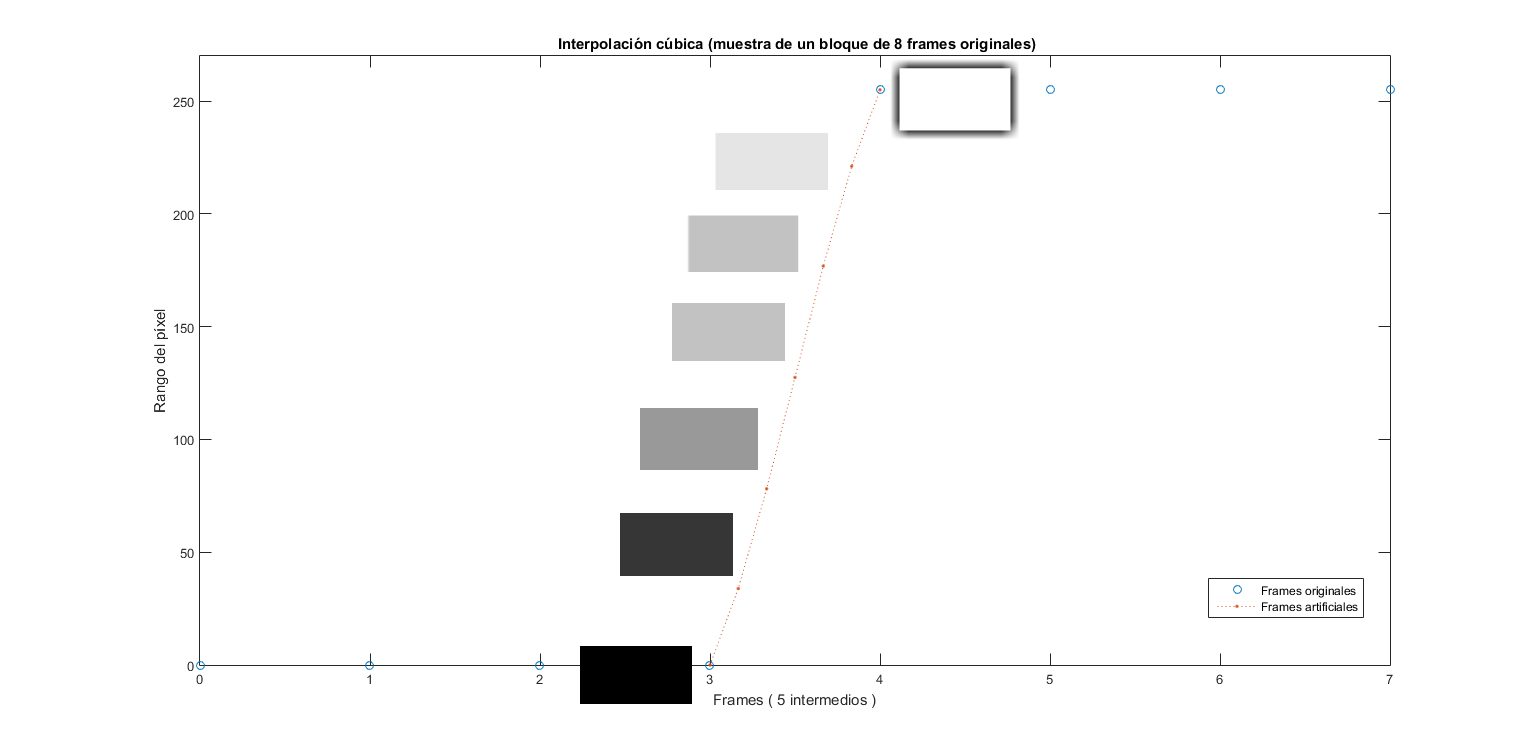
\includegraphics[width=0.75\textwidth]{GraficoSplines.png}
     \caption{Muestra del bloque que contiene el cambio, con los cuadros comparados}\label{fig:splineValidacion}
\end{figure}
\noindent

%---------------------------------------------------------------
\subsubsection{C\'amara Fija - Im\'agen Fija}

Equivalente a pensar que una im\'agen est\'a siendo reproducida durante un lapso de tiempo, que difiere al hecho de que una c\'amara est\'e quieta, enfocando a un objeto que puede ser sofocado por la luz. Y est\'a claro que el mero hecho de querer alentizar un video de tal caracter\'istica, solo servir\'a para aumentar la duraci\'on de la misma. Por lo conceptualmente visto, no hay dudas de que si la implementaci\'on se realiz\'o de forma correcta, no existir\'ia ning\'un cambio en el video.

Usamos metodolog\'ias id\'enticas para los tres m\'etodos. Esto es, extraer cada cuadro artificial y corroborar que coincide con la foto utilizada.

\subsubsection*{\bf{Resultado:}}

Como en cada p\'ixel $(i,j)$ el valor se mantuvo constante, as\'i lo fue con las funciones interpoladoras. De esta manera, cualquier punto que era evaluado por m\'as frames que se le quisiese acomodar, solo produc\'ia un video m\'as largo. En conclusi\'on, la im\'agen permeneci\'o intacta durante toda su reproducci\'on.


%---------------------------------------------------------------
\subsection{Tiempos de ejecuci\'on}

%---------------------------------------------------------------
\subsection{C\'amara Fija - Im\'agen Fija}

%---------------------------------------------------------------
\subsection{C\'amara Fija - Im\'agen M\'ovil}

%---------------------------------------------------------------
\subsection{C\'amara M\'ovil - Im\'agen Fija}

%---------------------------------------------------------------
\subsection{C\'amara M\'ovil - Im\'agen M\'ovil}

%---------------------------------------------------------------
\subsection{An\'alisis por M\'etodo en funci\'on del Video}

%---------------------------------------------------------------
\subsection{Artifacts}

%---------------------------------------------------------------
\subsection*{Experimentos a Futuro}
